\documentclass{article}
\usepackage{graphicx, tikz-cd, float, titlepic, booktabs} % Required for inserting images
\usepackage{pgfplots}
\pgfplotsset{compat=1.15}
\usepackage{mathrsfs}
\usetikzlibrary{arrows}
\usepackage{amsmath, amssymb, amsthm, amsfonts, siunitx, physics, gensymb}
\AtBeginDocument{\RenewCommandCopy\qty\SI}
\usepackage[version=4]{mhchem}
\usepackage[most,many,breakable]{tcolorbox}
\usepackage{xcolor, fancyhdr, varwidth}
\usepackage[Glenn]{fncychap}
%Options: Sonny, Lenny, Glenn, Conny, Rejne, Bjarne, Bjornstrup
\usepackage{hyperref, cleveref}
\usepackage{icomma, enumitem} %comma as decimal and continue enumerate with [resume]
\usepackage[danish]{babel}
%%%%%%%%%%%%%%%%%%%%%%%%%%%%%%
% SELF MADE COLORS
%%%%%%%%%%%%%%%%%%%%%%%%%%%%%%
\definecolor{myg}{RGB}{56, 140, 70}
\definecolor{myb}{RGB}{45, 111, 177}
\definecolor{myr}{RGB}{199, 68, 64}
\definecolor{mytheorembg}{HTML}{F2F2F9}
\definecolor{mytheoremfr}{HTML}{00007B}
\definecolor{mylenmabg}{HTML}{FFFAF8}
\definecolor{mylenmafr}{HTML}{983b0f}
\definecolor{mypropbg}{HTML}{f2fbfc}
\definecolor{mypropfr}{HTML}{191971}
\definecolor{myexamplebg}{HTML}{F2FBF8}
\definecolor{myexamplefr}{HTML}{88D6D1}
\definecolor{myexampleti}{HTML}{2A7F7F}
\definecolor{mydefinitbg}{HTML}{E5E5FF}
\definecolor{mydefinitfr}{HTML}{3F3FA3}
\definecolor{notesgreen}{RGB}{0,162,0}
\definecolor{myp}{RGB}{197, 92, 212}
\definecolor{mygr}{HTML}{2C3338}
\definecolor{myred}{RGB}{127,0,0}
\definecolor{myyellow}{RGB}{169,121,69}
\definecolor{myexercisebg}{HTML}{F2FBF8}
\definecolor{myexercisefg}{HTML}{88D6D1}
%%%%%%%%%%%%%%%%%%%%%%%%%%%%%%%%%%%%%%%%%%%%%%%%%%%%%%%%%%%%%%%%%%%%%%
% Box environments for theorems and problems
%%%%%%%%%%%%%%%%%%%%%%%%%%%%%%%%%%%%%%%%%%%%%%%%%%%%%%%%%%%%%%%%%%%%%
\setlength{\parindent}{1cm}
%================================
% Question BOX
%================================
\makeatletter
\newtcbtheorem{question}{Opgave}{enhanced,
	breakable,
	colback=white,
	colframe=myb!80!black,
	attach boxed title to top left={yshift*=-\tcboxedtitleheight},
	fonttitle=\bfseries,
	title={#2},
	boxed title size=title,
	boxed title style={%
			sharp corners,
			rounded corners=northwest,
			colback=tcbcolframe,
			boxrule=0pt,
		},
	underlay boxed title={%
			\path[fill=tcbcolframe] (title.south west)--(title.south east)
			to[out=0, in=180] ([xshift=5mm]title.east)--
			(title.center-|frame.east)
			[rounded corners=\kvtcb@arc] |-
			(frame.north) -| cycle;
		},
	#1
}{def}
\makeatother
%================================
% DEFINITION BOX
%================================

\newtcbtheorem[]{Definition}{Definition}{enhanced,
	before skip=2mm,after skip=2mm, colback=red!5,colframe=red!80!black,boxrule=0.5mm,
	attach boxed title to top left={xshift=1cm,yshift*=1mm-\tcboxedtitleheight}, varwidth boxed title*=-3cm,
	boxed title style={frame code={
					\path[fill=tcbcolback]
					([yshift=-1mm,xshift=-1mm]frame.north west)
					arc[start angle=0,end angle=180,radius=1mm]
					([yshift=-1mm,xshift=1mm]frame.north east)
					arc[start angle=180,end angle=0,radius=1mm];
					\path[left color=tcbcolback!60!black,right color=tcbcolback!60!black,
						middle color=tcbcolback!80!black]
					([xshift=-2mm]frame.north west) -- ([xshift=2mm]frame.north east)
					[rounded corners=1mm]-- ([xshift=1mm,yshift=-1mm]frame.north east)
					-- (frame.south east) -- (frame.south west)
					-- ([xshift=-1mm,yshift=-1mm]frame.north west)
					[sharp corners]-- cycle;
				},interior engine=empty,
		},
	fonttitle=\bfseries,
	title={#2},#1}{def}
\newtcbtheorem[]{definition}{Definition}{enhanced,
	before skip=2mm,after skip=2mm, colback=red!5,colframe=red!80!black,boxrule=0.5mm,
	attach boxed title to top left={xshift=1cm,yshift*=1mm-\tcboxedtitleheight}, varwidth boxed title*=-3cm,
	boxed title style={frame code={
					\path[fill=tcbcolback]
					([yshift=-1mm,xshift=-1mm]frame.north west)
					arc[start angle=0,end angle=180,radius=1mm]
					([yshift=-1mm,xshift=1mm]frame.north east)
					arc[start angle=180,end angle=0,radius=1mm];
					\path[left color=tcbcolback!60!black,right color=tcbcolback!60!black,
						middle color=tcbcolback!80!black]
					([xshift=-2mm]frame.north west) -- ([xshift=2mm]frame.north east)
					[rounded corners=1mm]-- ([xshift=1mm,yshift=-1mm]frame.north east)
					-- (frame.south east) -- (frame.south west)
					-- ([xshift=-1mm,yshift=-1mm]frame.north west)
					[sharp corners]-- cycle;
				},interior engine=empty,
		},
	fonttitle=\bfseries,
	title={#2},#1}{def}

\newtcbtheorem{theo}%
    {Theorem}{}{theorem}
\newtcolorbox{prob}[1]{colback=red!5!white,colframe=red!50!black,fonttitle=\bfseries,title={#1}}
%================================
% NOTE BOX
%================================

\usetikzlibrary{arrows,calc,shadows.blur}
\tcbuselibrary{skins}
\newtcolorbox{note}[1][]{%
	enhanced jigsaw,
	colback=gray!20!white,%
	colframe=gray!80!black,
	size=small,
	boxrule=1pt,
	title=\textbf{Note:},
	halign title=flush center,
	coltitle=black,
	breakable,
	drop shadow=black!50!white,
	attach boxed title to top left={xshift=1cm,yshift=-\tcboxedtitleheight/2,yshifttext=-\tcboxedtitleheight/2},
	minipage boxed title=1.5cm,
	boxed title style={%
			colback=white,
			size=fbox,
			boxrule=1pt,
			boxsep=2pt,
			underlay={%
					\coordinate (dotA) at ($(interior.west) + (-0.5pt,0)$);
					\coordinate (dotB) at ($(interior.east) + (0.5pt,0)$);
					\begin{scope}
						\clip (interior.north west) rectangle ([xshift=3ex]interior.east);
						\filldraw [white, blur shadow={shadow opacity=60, shadow yshift=-.75ex}, rounded corners=2pt] (interior.north west) rectangle (interior.south east);
					\end{scope}
					\begin{scope}[gray!80!black]
						\fill (dotA) circle (2pt);
						\fill (dotB) circle (2pt);
					\end{scope}
				},
		},
	#1,
}

%%%%%%%%%%%%%%%%%%%%%%%%%%%%%%%%%%%%%%%%%%%%%%%%%%%%%%%%%%%%%%%%%
% SELF MADE COMMANDS
%%%%%%%%%%%%%%%%%%%%%%%%%%%%%%
\newcommand{\sol}{\setlength{\parindent}{0cm}\textbf{\textit{Løsning:}}\setlength{\parindent}{1cm}}
%%%%%%%%%%%%%%%%%%%%%%%%%%%%%%%%%
\usepackage[tmargin=2cm,rmargin=1in,lmargin=1in,margin=0.85in,bmargin=2cm,footskip=.2in]{geometry}\pagestyle{fancy}
\lhead{Minrui Kevin Zhou 2.b}
\rhead{2.g terminsprøve mat}

\title{2.g Terminsprøve matematik\\
{\Large \textbf{2.b mat A}}}
\author{Kevin Zhou}
\date{\today}

\begin{document}
\maketitle
\section*{Bedømmelseskriterier:}
\begin{itemize}
    \setlength\itemsep{3cm}
    \Large
    \item  Redegørelse og dokumentation for metode
    \item Figurer, grafer og andre illustrationer
    \item Notation og layout
    \item Formidling og forklaring
\end{itemize}
\pagebreak
\begin{question}{Opgave 9}{}
  En person kaster en basketbold meget hårdt mod jorden. 
  Bolden rammer jorden i punktet $P$, hvorfra bolden hopper op igen.
  I modellen antages, at boldens højde som funktion af dens vandrette afstand fra $P$ kan skrives på formen
  \[
  f(x)= ax^2+bx+c
  \] 
  hvor $f(x)$ er boldens højde over jorden (målt i cm), når dens vandrette afstand fra $P$ er $x$ cm. 
  \begin{itemize}
    \item[a.] Bestem ved brug af alle tabellens 109 punkter værdierne af konstanterne $a,b$ og $c$. 
    \item[b.] Bestem boldens største højde over jorden ifølge modellen ved brug af $f'(x)$.
    \item[c.] Bestem den spidse vinkel, som tangenten til grafen for $f$ danner med vandret, når bolden igen rammer jorden.
  \end{itemize}
\end{question}
\sol \\
\textbf{a.} Vi laver en regressionsanalyse med mindste kvadraters metode via LoggerPro, hvilket kan ses i \cref{fig:bold}.
\begin{figure}[H]
\begin{center}
  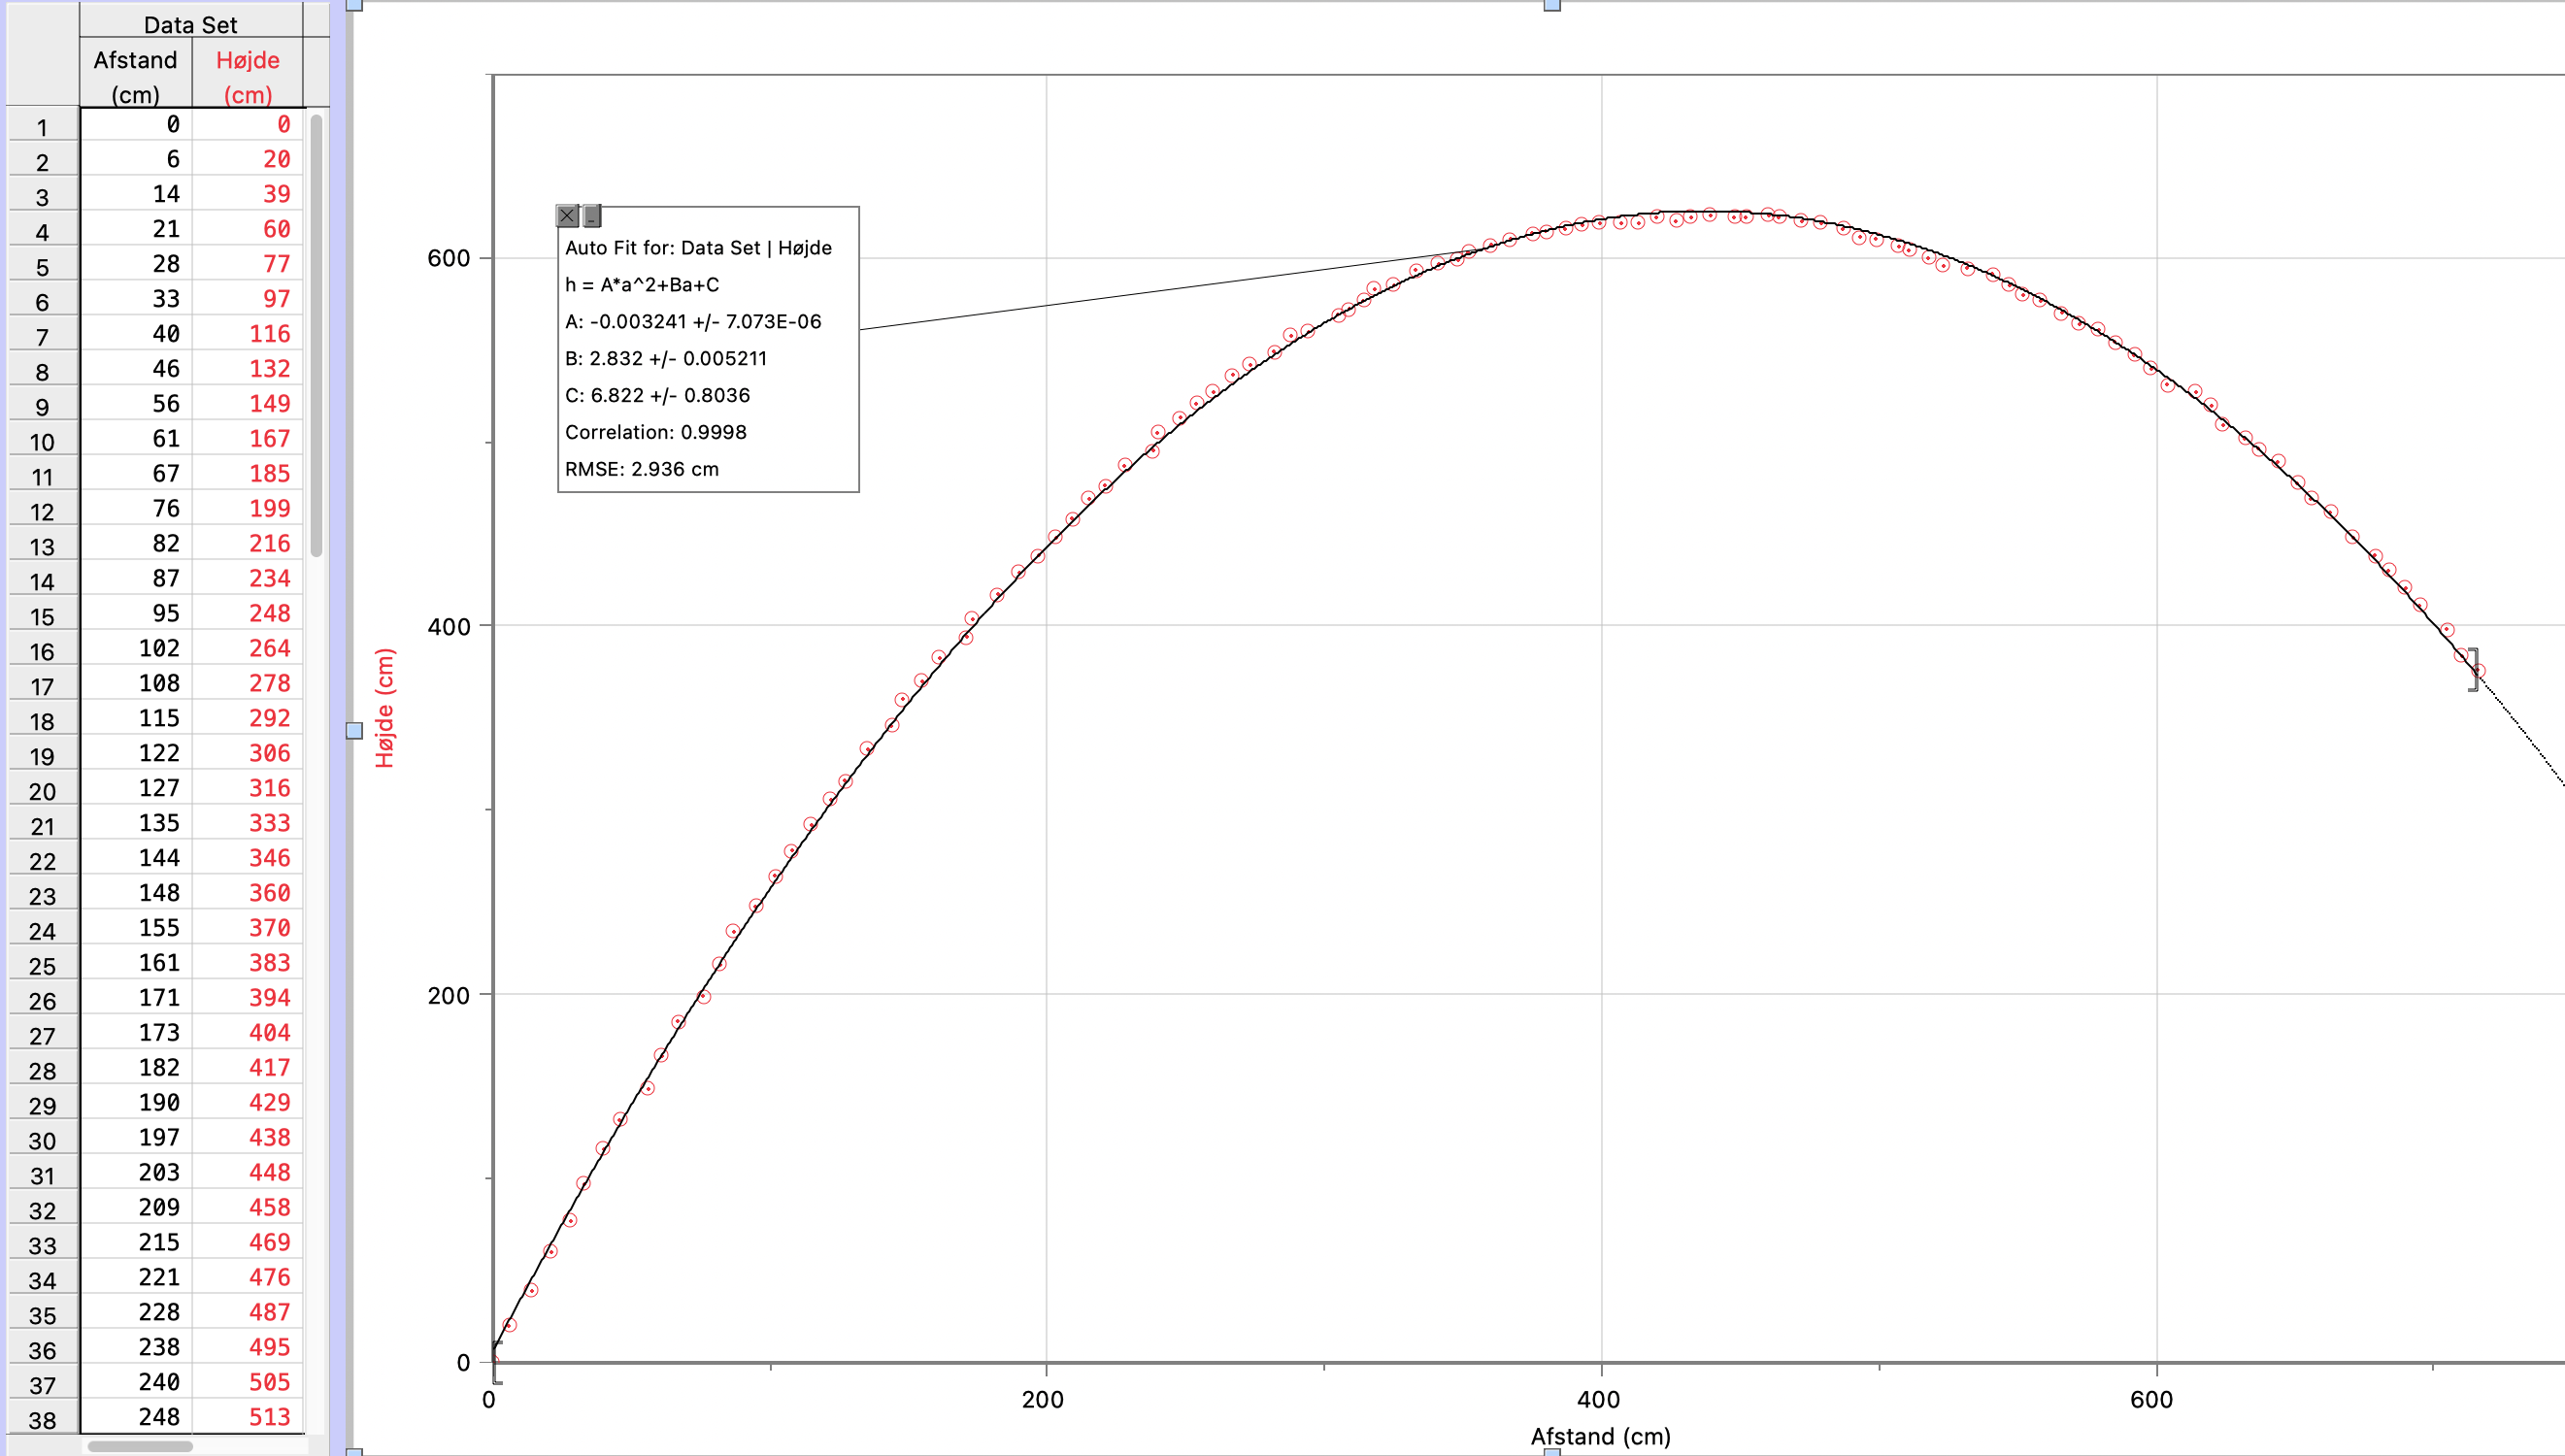
\includegraphics[width=\textwidth]{bold.png}
\end{center}
\caption{Regressionsanalyse lavet i LoggerPro}
\label{fig:bold}
\end{figure}
Vi får da konstanterne til at være
\begin{equation*}
\begin{split}
  a&=-0,003214\\ 
  b&=2,832\\ 
  c&=6,822
\end{split}
\end{equation*}
\textbf{b.}
Vi finder først den afledede funktion for $f$.
\begin{equation*}
\begin{split}
f'(x)&=2 \cdot (-0,003214x) +2,832\\
  &=-0,006428x + 2,832
\end{split}
\end{equation*}
Denne må være lig med 0 når højden er størst.
\begin{equation*}
\begin{split}
  f'(x)=0 &\implies -0,006428x + 2,832=0\\ 
  &\iff x=\frac{2,832}{0,006428}\approx 440,6
\end{split}
\end{equation*}
Vi tager da funktionen $f$ af denne $x$-værdi. 
\begin{equation*}
\begin{split}
  f\left(\frac{2,832}{0,006428}\right) \approx 630,67
\end{split}
\end{equation*}
Altså er den største højde over jorden ifølge modellen $630,67 \;\unit{cm} $.\\[1ex]
\textbf{c.}
Med CAS får vi, at den større rod for $f$ er $\frac{90 \sqrt{62561170} +708000}{1607}$. 
Vi tager den afledede funktion for $f$ af denne for at finde hældningen. 
Den spidse vinkel med vandret må så være den inverse tangent af hældningen.
\begin{equation*}
\begin{split}
  v&=\tan^{-1}\left(f'\left(\frac{90 \sqrt{62561170} +708000}{1607}\right)\right) \\ 
  &\approx -70,65 \degree 
\end{split}
\end{equation*}
Altså er den spidse vinkel dannet med vandret $-70,65 \degree$.
CAS-udklip ses i \cref{fig:CAS}
\begin{figure}[H]
\begin{center}
  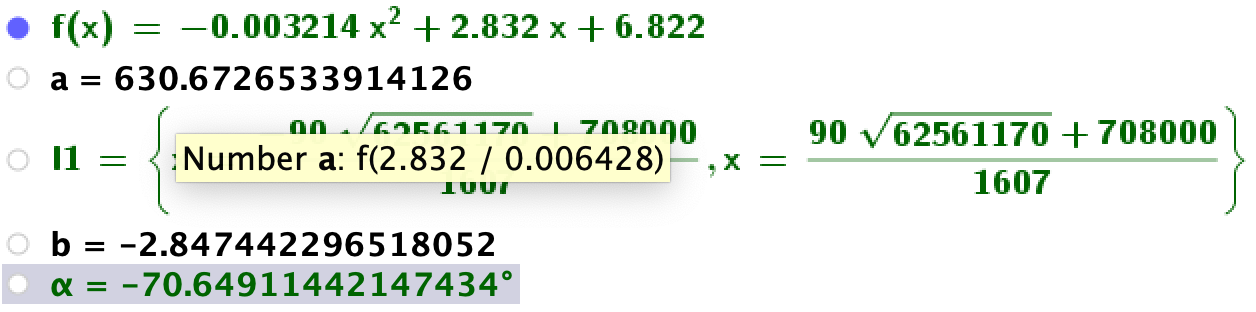
\includegraphics[scale=0.5]{CAS.png}
\end{center}
\caption{CAS-udklip}
\label{fig:CAS}
\end{figure}
\begin{question}{Opgave 10}{}
  I en model for vanddybden i en bestemt havn i løbet af et døgn er vanddybden $h(x)$
(målt i meter) til tiden $x$ (målt i antal timer efter midnat) givet ved
\[
  h(x)=2 \cdot \sin \left(\frac{\pi}{12}x\right) +7, \quad 0 \leq x < 24
\] 
\begin{itemize}
  \item[a.] Bestem den minimale vanddybde i havnen i løbet af døgnet.
  \item[b.] Bestem de tidspunkter på døgnet, hvor vanddybden i havnen er 8 meter.
\end{itemize}
\end{question}
\sol \\
\textbf{a.}
Vanddybden må være mindst, når $\sin\left(\frac{\pi}{12}x\right)$ er mindst. 
Dette er tilfældet når $\sin\left(\frac{\pi}{12}x\right)=-1$, hvilket vi ser godt kan lade sig gøre med definitionsmængden. 
Der er vanddybden
\[
2 \cdot (-1)+7 =5
\] 
Altså er den minimale vanddybde i havnen $5 \;\unit{m} $.\\[1ex]
\textbf{b.}
Vi løser da ligningen $h(x)=8$.
\begin{equation*}
\begin{split}
  2 \cdot \sin\left(\frac{\pi}{12}x\right)+7=8 \iff \sin\left(\frac{\pi}{12}x\right)=\frac{1}{2}
\end{split}
\end{equation*}
Med vores definitionsmængde er der to løsninger.
\begin{equation*}
\begin{split}
  \sin\left(\frac{\pi}{12}x\right)=\frac{1}{2} &\implies \frac{\pi}{12}x = \sin^{-1}\left(\frac{1}{2}\right)\lor \frac{\pi}{12}x= \pi- \sin^{-1}\left(\frac{1}{2}\right) \\ 
  &\iff x=2 \lor x=10
\end{split}
\end{equation*}
Altså er vanddybden 8 meter klokken 2 og klokken 10. 
Dette stemmer overens med funktionens graf, der ses i \cref{fig:vand}.
\begin{figure}[H]
\begin{center}
  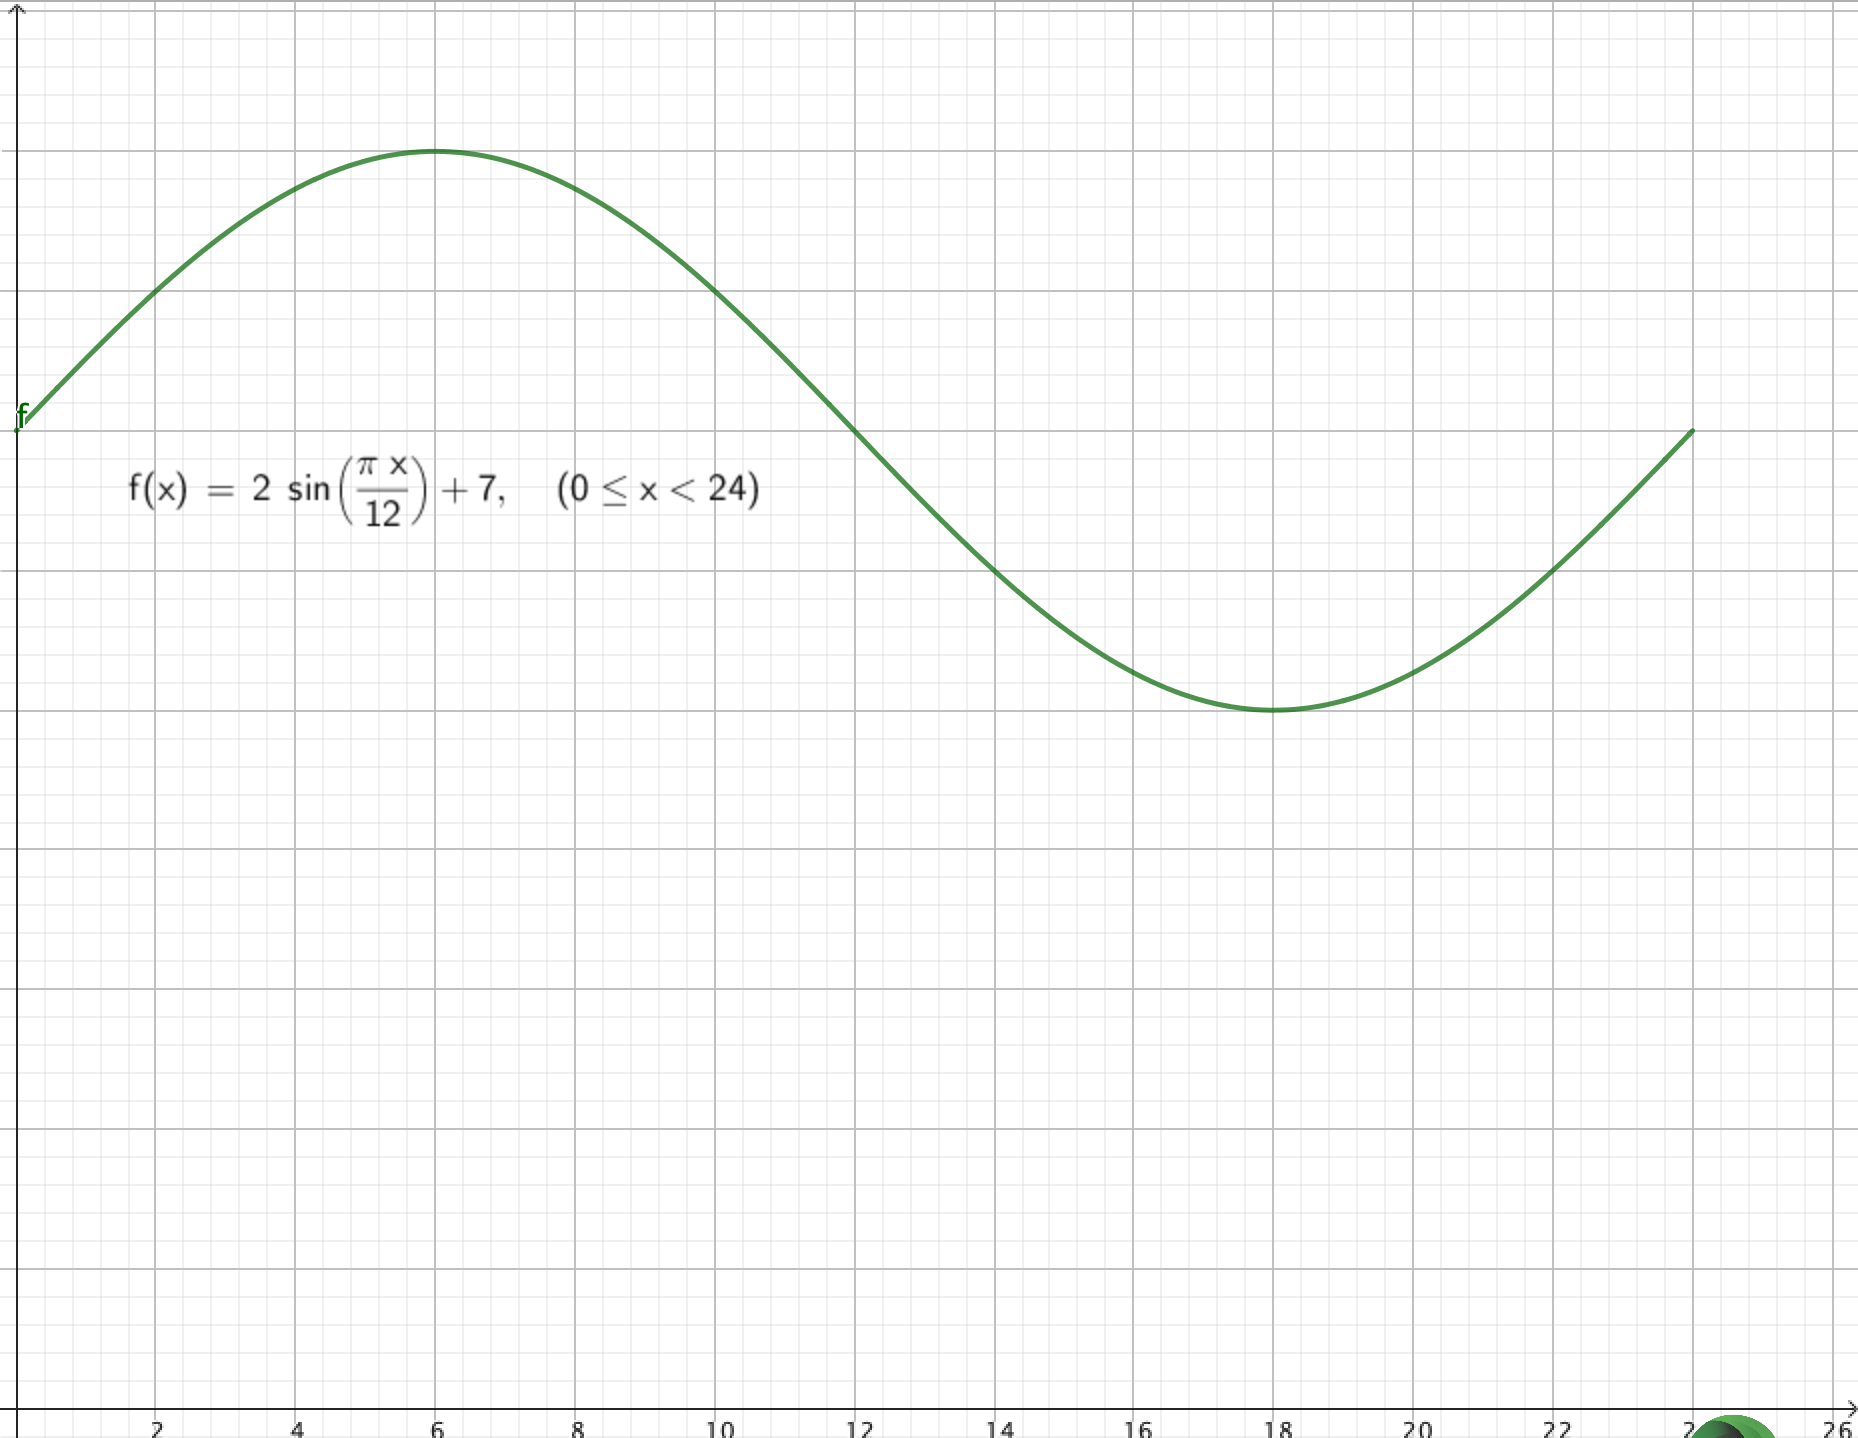
\includegraphics[width=\textwidth]{vand.png}
\end{center}
  \caption{Grafen for $h$}
\label{fig:vand}
\end{figure}
\begin{question}{Opgave 11}{}
  I en model kan udviklingen af den årlige nedbørsmængde i en bestemt by beskrives ved
  \[
  780 \cdot e^{0,012x}
  \] 
  hvor $f(x)$ betegner den årlige nedbørsmængde (målt i mm) og $x$ betegner tiden målt
i antal år efter 2020. 
\begin{itemize}
  \item[a.] Benyt modellen til at bestemme det årstal, hvor den årlige nedbørsmængde
overstiger $1000 \;\unit{mm} $.
\item[b.] Bestem $f'(5)$, og giv en fortolkning af dette tal.
\end{itemize}
\end{question}
\sol \\
\textbf{a.}
Vi løser da ligningen $f(x)=1000$.
\begin{equation*}
\begin{split}
  f(x)=1000 &\implies 780 \cdot e^{0,012x}=1000\\
  &\iff x=\frac{\ln \left(\frac{50}{39}\right) }{0,012} \approx 20,7
\end{split}
\end{equation*}
Altså overstiger den årlige nedbørsmængde $1000 \;\unit{mm} $ i år 2040. \\[1ex]
\textbf{b.}
Vi finder først den afledede funktion for $f$. 
\begin{equation*}
\begin{split}
  f'(x)&=0,012 \cdot 780 \cdot e^{0,012x}\\ 
  &=9,36 \cdot e^{0,012x}
\end{split}
\end{equation*}
Vi tager nu den afledede funktion af $5$.
\begin{equation*}
\begin{split}
  f'(5)&=9,36 \cdot e^{0,012 \cdot 5}\\ 
  &\approx 9,94
\end{split}
\end{equation*}
Dette tal fortæller, at det årlige nedbør vokser med $9,94 \;\unit{mm} $ per år ved tiden $x=5$. 
\begin{question}{Opgave 12}{}
  I et koordinatsystem er der givet et punkt $C(10,-2)$ og en linje $l$ med ligningen 
  \[
  4x+3y-6=0
  \] 
\begin{itemize}
  \item[a.] Benyt en formel til at bestemme afstanden fra $C$ til $l$. 
\end{itemize}
En cirkel har centrum i $C$ og radius 3.
Det punkt, som ligger på cirklen, og som har den mindste afstand til $l$, kaldes for $P$.
\begin{itemize}
  \item[b.] Bestem koordinatsættet til punktet $P$.
\end{itemize}
\end{question}
\sol \\
\textbf{a.}
Siden der gælder, at afstanden fra et punkt $(x_1,y_1)$ til en linje med ligningen $ax+by+c=0$ er 
\[
\frac{\abs{a \cdot x_1 + b \cdot y_1 + c} }{\sqrt{a^2+b^2} }
\] 
 så gælder der i dette tilfælde, at afstanden fra $C$ til $l$ må være
\[
\frac{\abs{4 \cdot 10 + 3 \cdot (-2)-6} }{\sqrt{4^2+3^2} }=\frac{28}{5}
\] 
\textbf{b.}
Da der kun er et punkt $P$, så må der gælde, at afstanden til linjen må være 3 mindre end ved $C$.
Siden cirklen ikke skærer linjen, så kan vi udelade den absolutte værdi i tælleren.
\begin{equation*}
\begin{split}
  \frac{4 \cdot x + 3 \cdot y -6}{5}=\frac{13}{5}&\iff x=\frac{19-3y}{4}
\end{split}
\end{equation*}
Vi substituerer ind i cirklens ligning og løser den med CAS.
\begin{equation*}
\begin{split}
  \left(\frac{19-3y}{4}-10\right)^2+(y+2)^2=3^2 \iff y=\frac{-19}{5}
\end{split}
\end{equation*}
Vi regner nu $x$-koordinatet ud.
\[
x=\frac{19-3 \cdot \frac{-19}{5}}{4}=\frac{38}{5}
\] 
Altså har vi
\[
P=\left(\frac{38}{5},\frac{-19}{5}\right) 
\] 
\begin{question}{Opgave 14}{}
  En klods skal være fire gange så lang, som den er bred. Klodsens rumfang skal være $200 \;\unit{cm^3} $.
  \begin{itemize}
    \item[a.] Opstil en formel for klodsens højde udtrykt ved klodsens bredde.
    \item[b.] Bestem hvilken bredde, længde og højde, klodsen skal have, når klodsens
overfladeareal skal være mindst muligt.
  \end{itemize}
\end{question}
\sol \\
\textbf{a.}
Vi har at
\begin{equation*}
\begin{split}
  4b^2 \cdot h=200 \iff h= \frac{200}{4b^2}
\end{split}
\end{equation*}
hvor $b$ er klodsens bredde og $h$ er klodsens højde. \\[1ex]
\textbf{b.}
Vi finder først et udtryk for halvdelen af klodsens overfladeareal
\begin{equation*}
\begin{split}
  A&=4b^2+\frac{200b}{4b^2} + \frac{200 \cdot 4b}{4b^2}\\ 
  &=4b^2+\frac{250}{b}
\end{split}
\end{equation*}
Vi differentierer dette udtryk.
\begin{equation*}
\begin{split}
  \dv{b}\left(4b^2+\frac{250}{b}\right)=8b-\frac{250}{b^2}
\end{split}
\end{equation*}
Vi sætter dette udtryk lig 0 og løser for $b$.
\begin{equation*}
\begin{split}
  8b-\frac{250}{b^2}=0 &\iff 8b^3=250\\ 
  &\iff b=\left(\frac{250}{8}\right)^{\frac{1}{3}} \approx 3,15
\end{split}
\end{equation*}
Altså er bredden $3,15 \;\unit{cm} $.
Længden må være $4 \cdot 3,15 \;\unit{cm} =12,6 \;\unit{cm} $.
Højden må da være $\frac{200 \;\unit{cm^3} }{4 \cdot (3,15 \;\unit{cm} )^2} \approx 5,04 \;\unit{cm} $.
\end{document}
